\documentclass[11pt,a4paper]{ctexart}

\usepackage{amsmath,amssymb,bm}
\usepackage{geometry}
\usepackage{enumitem}
\usepackage{fancyhdr}
\usepackage{lastpage}
\usepackage{xcolor}
\usepackage{tcolorbox}
\usepackage{tikz}
\usepackage{titlesec}
\usepackage{microtype}
\usepackage{graphicx}
\usepackage{esint}
\usetikzlibrary{arrows.meta,calc}

\geometry{left=2.15cm,right=2.15cm,top=2.0cm,bottom=2.0cm}
\setlength{\parindent}{2em}
\setlength{\parskip}{0.25em}
\linespread{1.12}
\graphicspath{{figures/}}

\definecolor{mainblue}{RGB}{39,91,150}
\definecolor{lightblue}{RGB}{232,241,252}
\definecolor{darkgray}{RGB}{65,65,65}
\definecolor{lightgray}{RGB}{245,246,248}

\titleformat{\section}{\large\bfseries\color{mainblue}}{}{0em}{}[\titlerule]
\titleformat{\subsection}{\normalsize\bfseries\color{darkgray}}{}{0em}{}
\titlespacing*{\section}{0pt}{0.9em}{0.45em}
\titlespacing*{\subsection}{0pt}{0.65em}{0.25em}

\setlist[enumerate]{leftmargin=2.2em,itemsep=0.25em,topsep=0.25em}
\setlist[itemize]{leftmargin=2.0em,itemsep=0.2em,topsep=0.2em}

\pagestyle{fancy}
\fancyhf{}
\lhead{\small 格物助航｜每日一练}
\rhead{\small 2026.6.15}
\cfoot{\small 第 \thepage\ 页 / 共 \pageref{LastPage} 页}
\renewcommand{\headrulewidth}{0.4pt}

\newtcolorbox{problemBox}{
  colback=lightblue,
  colframe=mainblue,
  arc=2mm,
  boxrule=0.7pt,
  left=1.0em,
  right=1.0em,
  top=0.8em,
  bottom=0.8em,
  before skip=0.6em,
  after skip=0.8em
}

\newtcolorbox{tipBox}{
  colback=lightgray,
  colframe=darkgray,
  arc=1.5mm,
  boxrule=0.5pt,
  left=0.9em,
  right=0.9em,
  top=0.6em,
  bottom=0.6em,
  before skip=0.5em,
  after skip=0.5em
}

\newcommand{\dd}{\mathrm{d}}

\begin{document}

\begin{center}
  {\Large\bfseries\color{mainblue} 格物助航｜每日一练}\par
  \vspace{0.25em}
  {\large 电磁学第二章：静电场中的导体和电介质}\par
  \vspace{0.35em}
  {\small 2026年6月15日}\par
  \vspace{0.35em}
  {\small 编写：罗琦皓}
\end{center}

\vspace{-0.3em}

\begin{problemBox}
\noindent\textbf{题目}\quad
一平行板电容器两极板面积为 $S$，板间距为 $d$，忽略边缘效应。真空时电容器接在电压为 $U_0$ 的电源上，设
\[
  C_0=\frac{\varepsilon_0S}{d},\quad
  Q_0=C_0U_0,\quad
  E_0=\frac{U_0}{d},\quad
  D_0=\varepsilon_0E_0,\quad
  W_0=\frac12 C_0U_0^2 .
\]
现把相对介电常量为 $\varepsilon_r$ 的各向同性均匀电介质充满两极板间。分别讨论：
\begin{enumerate}
  \item 甲：电容器始终与电源相连，极板间电压保持 $U_0$；
  \item 乙：先充电至 $U_0$ 后断开电源，再插入电介质。
\end{enumerate}
求两种情况下的 $C,Q,E,D,W$，并求介质表面极化电荷面密度的大小。
\end{problemBox}

\begin{center}
  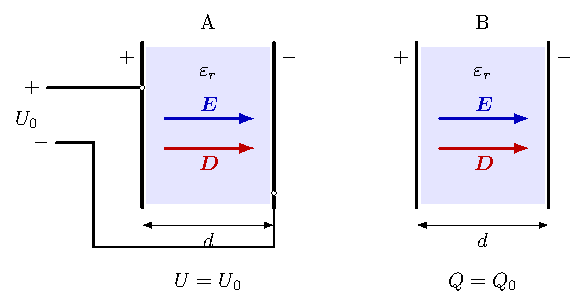
\includegraphics[width=0.68\textwidth]{dielectric_capacitor.pdf}\par
  {\small A 图中电源正、负端分别接两极板，保持 $U=U_0$；B 图为断电后的孤立电容器，保持 $Q=Q_0$。}
\end{center}

\section*{详细解法}

\subsection*{一、先抓住共同点}

电介质充满极板间后，平行板电容器的电容变为
\[
  C=\varepsilon_r C_0=\frac{\varepsilon_0\varepsilon_rS}{d}.
\]
对各向同性线性介质，有
\[
  \bm D=\varepsilon_0\varepsilon_r\bm E,
  \qquad
  \bm P=\varepsilon_0(\varepsilon_r-1)\bm E.
\]
其中 $\bm D$ 由自由电荷决定，$\bm E$ 是介质中的实际总电场，$\bm P$ 决定介质表面的极化电荷。

\subsection*{二、甲：保持与电源相连}

恒压意味着两极板电势差不变：
\[
  U_{\text{甲}}=U_0.
\]
所以
\[
  E_{\text{甲}}=\frac{U_0}{d}=E_0.
\]
电容增大为 $\varepsilon_rC_0$，因此极板上的自由电荷变为
\[
  Q_{\text{甲}}=C_{\text{甲}}U_0
  =\varepsilon_r C_0U_0
  =\varepsilon_r Q_0.
\]
于是
\[
  D_{\text{甲}}=\frac{Q_{\text{甲}}}{S}
  =\varepsilon_rD_0
  =\varepsilon_0\varepsilon_rE_0.
\]
储存的电场能为
\[
  W_{\text{甲}}
  =\frac12 C_{\text{甲}}U_0^2
  =\varepsilon_rW_0.
\]
极化强度大小为
\[
  P_{\text{甲}}
  =\varepsilon_0(\varepsilon_r-1)E_0,
\]
所以介质表面的极化电荷面密度大小为
\[
  \boxed{\sigma'_{\text{甲}}=\varepsilon_0(\varepsilon_r-1)E_0.}
\]
靠近正极板的一面为负极化电荷，靠近负极板的一面为正极化电荷。

\subsection*{三、乙：断开电源后插入介质}

断电后极板上的自由电荷不能再改变：
\[
  Q_{\text{乙}}=Q_0.
\]
因此
\[
  D_{\text{乙}}=\frac{Q_0}{S}=D_0.
\]
由 $\bm D=\varepsilon_0\varepsilon_r\bm E$ 得
\[
  E_{\text{乙}}
  =\frac{D_0}{\varepsilon_0\varepsilon_r}
  =\frac{E_0}{\varepsilon_r}.
\]
两极板间电压变为
\[
  U_{\text{乙}}=E_{\text{乙}}d
  =\frac{U_0}{\varepsilon_r}.
\]
储存的电场能为
\[
  W_{\text{乙}}
  =\frac{Q_0^2}{2C_{\text{乙}}}
  =\frac{Q_0^2}{2\varepsilon_rC_0}
  =\frac{W_0}{\varepsilon_r}.
\]
极化强度大小为
\[
  P_{\text{乙}}
  =\varepsilon_0(\varepsilon_r-1)\frac{E_0}{\varepsilon_r},
\]
所以
\[
  \boxed{\sigma'_{\text{乙}}
  =\frac{\varepsilon_r-1}{\varepsilon_r}\varepsilon_0E_0
  =\frac{\varepsilon_r-1}{\varepsilon_r}D_0.}
\]

\subsection*{四、结果汇总}

\[
\begin{array}{c|c|c}
 & \text{甲：恒压，}U=U_0 & \text{乙：断电，}Q=Q_0\\
\hline
C & \varepsilon_rC_0 & \varepsilon_rC_0\\
Q & \varepsilon_rQ_0 & Q_0\\
E & E_0 & E_0/\varepsilon_r\\
D & \varepsilon_rD_0 & D_0\\
W & \varepsilon_rW_0 & W_0/\varepsilon_r
\end{array}
\]

\section*{技巧与知识点}

\begin{tipBox}
\begin{enumerate}
  \item \textbf{先看约束量：}与电源相连时 $U$ 不变；断电后 $Q$ 不变。这一步决定全题方向。
  \item \textbf{$D$ 看自由电荷，$E$ 看介质：}平行板中 $D=\sigma_{\text{free}}$，再用 $D=\varepsilon_0\varepsilon_rE$ 求实际电场。
  \item \textbf{电容只由结构和介质决定：}介质充满后 $C=\varepsilon_rC_0$，与是否接电源无关。
  \item \textbf{能量公式要配套：}恒压常用 $W=\frac12CU^2$；定电荷常用 $W=\frac{Q^2}{2C}$。
  \item \textbf{极化电荷符号：}介质靠近正极板的一面出现负极化电荷，靠近负极板的一面出现正极化电荷。
\end{enumerate}
\end{tipBox}

\section*{复习建议}

第二章的复习重点不是背一串公式，而是先判断导体边界条件和电源状态。看到电容器题，先在题边写下“恒压”或“定电荷”；看到介质题，优先使用
\[
  \oiint \bm D\cdot \dd\bm S=\sum q_{\text{free}},
  \qquad
  \bm D=\varepsilon_0\varepsilon_r\bm E.
\]
再回到 $U=Ed$、$C=Q/U$、$W=\frac12CU^2=\frac{Q^2}{2C}$。这样可以同时处理选择题、填空题和计算题。

\end{document}
